%\clearpage
\section{Risultati}
\label{sec:risultati}
I programmi sono stati eseguiti mediante il seguente comando:
\begin{quotation}
\script{bash eserc\_lab.sh -a 20}
\end{quotation}
che esegue l'intero processo, generando 20 problemi simili per ogni incremento della densità dei nodi, pari a $10$, per le istanze \emph{casuali} e \emph{cluster}; mentre vengono generati solamente 20 problemi con istanze \emph{circolari} in quanto non è presente casualità nella loro generazione.

In totale sono quindi state generate $1020$ istanze, $200$ di tipo casuale, $800$ di tipo cluster e $20$ di tipo circolare.

I grafici riportano sull'asse delle ascisse il numero di nodi del problema, mentre sull'asse delle ordinate il tempo in secondi che è servito per trovare la soluzione, da notare che si è scelto di rappresentare il tempo in scala logaritmica.

I punti di interesse sono quelli identificati dal simbolo presente nella legenda di ogni grafico e rappresentano la media dei risultati ottenuti per le istanze simili, mentre le linee verticali indicano la variabilità nei risultati individuata tramite la deviazione standard.

\subsection{\acronimo{cplex}}

\begin{figure}[htb]
	\centering
	\begin{subfigure}[b]{.45\textwidth}
		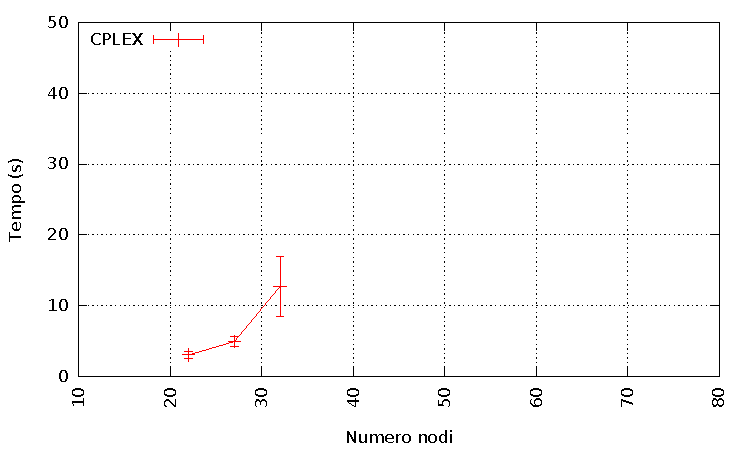
\includegraphics[width=\textwidth]{immagini/cplex_casuali.pdf}
		\caption{Istanze casuali}
		\label{fig:casuali cplex}
	\end{subfigure}
	\quad
	\begin{subfigure}[b]{.45\textwidth}
		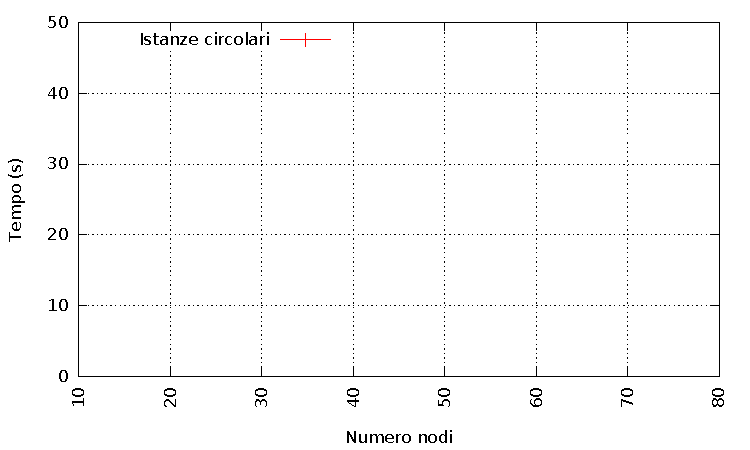
\includegraphics[width=\textwidth]{immagini/cplex_circolari.pdf}
		\caption{Istanze circolari}
		\label{fig:circolari cplex}
	\end{subfigure}
	\caption{Istanza casuali e circolari - \acronimo{cplex}}
	\label{fig:casuali circolari cplex}
\end{figure}

In figura \ref{fig:casuali cplex} vediamo i risultati per le istanze casuali, esse seguono un andamento abbastanza regolare con il crescere del numero dei nodi: per istanze piccole il tempo di risoluzione è abbastanza rapido, ma sale molto velocemente, fino a oltre $200s$, con l'aumentare dei nodi.

\begin{table}[htb]
	\footnotesize
	\centering
	\caption{Tempi e costi istanze casuali - \acronimo{cplex}}
	\label{tab:casuali}
	\begin{tabular}{cS[table-format=3.4]S[table-format=2.4]S[table-format=2.1]}
	\toprule
	\multirow{2}*{Numero nodi} 	& {Tempo medio} & {Deviazione standard} & \multirow{2}*{Costo medio} \\
								& {(s)}			& {(s)} 				& \\
	\midrule
	11	& 0.2438		& 0.1045	& 55.9 \\
	16	& 0.8337		& 0.3740	& 65.1 \\
	20	& 2.2390		& 1.6470	& 69.6 \\
	25	& 3.6030		& 1.2315	& 76.5 \\
	29	& 6.8557		& 3.9426	& 83.6 \\
	34	& 24.7649		& 13.2507	& 88.9 \\
	38	& 51.4854		& 25.8351	& 91.3 \\
	43	& 101.6627		& 33.2080	& 99.1 \\
	47	& 144.4995		& 24.6324	& 102.2 \\
	52	& 255.3258		& 65.0774	& 107.1 \\
	\bottomrule
	\end{tabular}
\end{table}

Per quanto riguarda le istanze circolari, vediamo in figura \ref{fig:circolari cplex} che i tempi sono molto più bassi rispetto alle istanze casuali: questo è dovuto alla semplicità intrinseca di queste istanze che sono quindi più facili da risolvere.
Da notare come l'andamento del grafico non sia molto lineare: questo fatto probabilmente è dovuto al carico del processore al momento dell'esecuzione del test, che può non essere stato costante durante il periodo di prova.

\begin{table}[htb]
	\footnotesize
	\centering
	\caption{Tempi e costi istanze circolari - \acronimo{cplex}}
	\label{tab:circolari}
	\begin{tabular}{cS[table-format=1.4]S[table-format=3.0]cS[table-format=1.4]S[table-format=3.0]}
	\toprule
	\multirow{2}*{Numero nodi} 	& {Tempo medio} & \multirow{2}*{Costo} 	& \multirow{2}*{Numero nodi} 	& {Tempo medio} & \multirow{2}*{Costo}\\
								& {(s)}			&  						& 								& {(s)}			&  \\
	\midrule
	8	& 0.1228	& 16 & 48	& 1.2384	& 96 \\
	12	& 0.1209	& 24 & 52	& 2.3079	& 104 \\
	16	& 0.0663	& 32 & 56	& 4.1274	& 112 \\
	20	& 0.2185	& 40 & 60	& 4.6480	& 120 \\
	24	& 0.3220	& 48 & 64	& 3.7191	& 128 \\
	28	& 0.2246	& 56 & 68	& 3.6495	& 136 \\
	32	& 0.4750	& 64 & 72	& 3.7701	& 144 \\
	36	& 0.8386	& 72 & 76	& 3.4811	& 152 \\
	40	& 1.8196	& 80 & 80	& 4.2138	& 160 \\
	44	& 1.2220	& 88 & 84	& 6.5727	& 168 \\
	\bottomrule
	\end{tabular}
\end{table}

Tutti i tempi e i costi medi ottenuti sono visibili nella tabella \ref{tab:casuali} per le istanze casuali e in tabella \ref{tab:circolari} per quelle circolari.
Il costo medio per le istanze casuali non è molto significativo in quanto il simplesso è un algoritmo esatto e ogni istanza è diversa dall'altra, di conseguenza il costo esatto delle rispettive soluzioni è diverso.
Tale media verrà però utilizzata per fare un confronto con \tabu in modo da valutare la bontà delle soluzioni trovate da tale metaeuristica.

\begin{figure}[htb]
	\centering
	\begin{subfigure}[b]{.45\textwidth}
		\includegraphics[width=\textwidth]{immagini/cplex_cluster_1.pdf}
		\caption{Istanze 1 cluster}
	\end{subfigure}
	\quad
	\begin{subfigure}[b]{.45\textwidth}
		\includegraphics[width=\textwidth]{immagini/cplex_cluster_2.pdf}
		\caption{Istanze 2 cluster}
	\end{subfigure}
	\\
	\begin{subfigure}[b]{.45\textwidth}
		\includegraphics[width=\textwidth]{immagini/cplex_cluster_3.pdf}
		\caption{Istanze 3 cluster}
	\end{subfigure}
	\quad
	\begin{subfigure}[b]{.45\textwidth}
		\includegraphics[width=\textwidth]{immagini/cplex_cluster_4.pdf}
		\caption{Istanze 4 cluster}
	\end{subfigure}
	\caption{Istanze cluster - \acronimo{cplex}}
	\label{fig:cluster cplex}
\end{figure}

In figura \ref{fig:cluster cplex} sono riportati i grafici riguardanti le istanze cluster: si può notare come abbiano tutti un andamento simile con tempi di risoluzione comparabili eccezion fatta per le istanze con $2$ nodi a $1$ cluster che hanno richiesto un tempo molto inferiore.

L'unico aspetto da sottolineare è la deviazione standard molto alta sulle istanze con $32$ nodi a $2$ cluster che è dovuta probabilmente ad un'istanza particolare che ha richiesto un tempo di risoluzione molto superiore alle altre.

\begin{figure}[htb]
	\centering
	\includegraphics[width=.85\textwidth]{immagini/cplex_all.pdf}
	\caption{Istanze casuali, cluster e circolari - \script{cplex}}
	\label{fig:all cplex}
\end{figure}

Infine ho deciso di riportare un grafico completo di tutti i risultati ottenuti, questo è visibile in figura \ref{fig:all cplex}.
È possibile vedere come con ogni tipologia di istanza, tranne quelle circolari, a parità di numero di nodi e quindi di complessità del problema, le prestazioni del programma siano simili.

È presente solo un leggero aumento nei tempi per quanto riguarda le istanze a $2$ cluster: esse infatti sono costruite utilizzando due quarti opposti della griglia, creando quindi maggiori difficoltà nella risoluzione in quanto i nodi si trovano in due zone distanti e separate fra loro.
Nei casi con $3$ e $4$ cluster invece la griglia ha una quantità di nodi maggiori ed è meno evidente la separazione tra gli stessi cluster.

Nella tabella \ref{tab:cluster} in appendice \ref{sec:tabelle} sono riportati i tempi medi e i costi medi per la risoluzione delle istanze cluster.

\subsection{Tabu Search}

Ho scelto di utilizzare la metaeuristica \tabu per risolvere solo alcuni dei problemi generati precedentemente: mi sono concentrato infatti sulle istanze generate casualmente; dal momento che la mia implementazione presenta una generazione della soluzione di partenza randomizzata, ho risolto $10$ volte ogni istanza in modo da avere dati statistici apprezzabili.

La \tabu ha un parametro chiamato \emph{tabu tenure} che permette di determinare la lunghezza della \emph{tabu list} determinando quindi, quando settato in modo appropriato, un miglioramento per quanto riguarda il valore della soluzione trovata, che dovrebbe avvicinarsi maggiormente al valore esatto calcolato da \acronimo{cplex}.

Il modo migliore per testare questa caratteristica mi è sembrato quello di effettuare la risoluzione delle istanze con diversi valori e riportarle su grafico in modo da capire i miglioramenti ottenuti.
Ho scelto di provare i valori di \emph{tabu tenure} tra $4$ e $8$, dato che erano i valori suggeriti per la dimensione dei problemi che ho usato.

\begin{figure}[htb]
	\centering
	\includegraphics[width=.85\textwidth]{immagini/tabu_all_tempo.pdf}
	\caption{Tempi istanze casuali - \tabu}
	\label{fig:all tempi tabu}
\end{figure}

In figura \ref{fig:all tempi tabu} è riportato il grafico complessivo relativo ai tempi di risoluzione dei problemi mediante l'algoritmo \tabu; si può notare subito come i tempi siano molto bassi rispetto a quanto visto per \acronimo{cplex} e seguano un andamento regolare.
Inoltre le prestazioni non cambiano con diversi valori di \emph{tabu tenure} come, infatti, ci si aspetta.

\begin{figure}[htb]
	\centering
	\includegraphics[width=.85\textwidth]{immagini/tabu_all_costo.pdf}
	\caption{Costi istanze casuali - \tabu}
	\label{fig:all costi tabu}
\end{figure}

In figura \ref{fig:all costi tabu}, invece, troviamo il grafico relativo alle medie dei costi delle soluzioni che sono state trovate: si può notare che al crescere del numero dei nodi si intravede un miglioramento con valori di \emph{tabu tenure} più alti, mentre con istanze di piccole dimensioni le differenze sono praticamente nulle.

Per avere un'idea precisa dei valori trovati si rimanda ai grafici in figura \ref{fig:tempi tabu} relativi ai tempi, a quelli in figura \ref{fig:costi tabu} relativi ai costi posti in appendice \ref{sec:grafici} e alla tabella \ref{tab:tabu} posta in appendice \ref{sec:tabelle} che riporta tutti i risultati ottenuti.